\section{Model Exercise 0-2 (13): Humidity controlled long-term bending test}
\label{sec:mex13}
%------------------------------------------------------------------------------
\Authors{Thomas Nagel}
%------------------------------------------------------------------------------
%------------------------------------------------------------------------------
\subsection{Experimental set-up}
%------------------------------------------------------------------------------
\begin{wrapfigure}{r}{10cm}
\centering
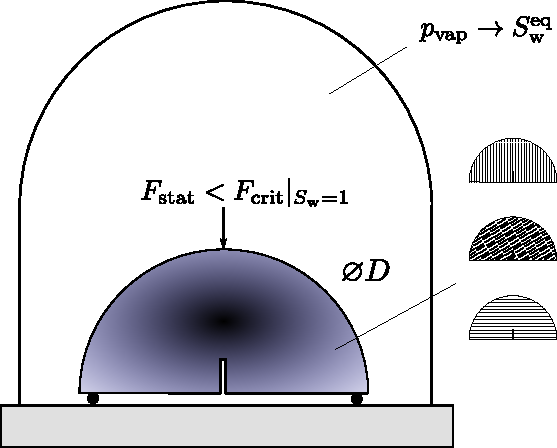
\includegraphics[width=10cm]{figures/GeomInt_MEx13.pdf}
\caption{Concept for a humidity controlled long-term bending test setup}
\label{fig:GeomInt_MEx13}
\end{wrapfigure}
The background for this proposal is the CD-A experiment in Mt. Terri in which cyclic humidity variations cause measurable fluctuations in the crack mouth opening. However, it is less well known whether this leads to crack closure or progressive crack growth. 

From a modelling perspective, the intention is to investigate more deeply several coupling effects in a H\textsuperscript{2}M setting. Thus, the focus is on Experiment B in the description below. Therefore, the test is defined as follows:

\begin{itemize}
	\item Three-point bending tests are performed on semi-cylindrical samples. the reason for the sample shape is simply an easier sample preparation compared to rectangular prismatic bars.
	\item In principle, anisotropy can be studied by using cores from appropriately aligned bore holes. Standard tests would allow studying orientation-dependent fracture toughness etc. (\textbf{Experiment A})
	\item The CMOD and the displacement of the load point should be measured. If possible, the full displacement field on the sample's face can be measured by optical methods.
	\item For \textbf{Experiment B}, the same setup is used but the samples are put into a desiccator (or other humidity-controlled environment).
	\item A static load (dead weight) is applied to a fully saturated sample which is \textit{sub-critical}, i.e. this load does not lead to immediate failure. If rate-dependent effects (creep) can be considered irrelevant, failure of the sample will not occur over time. This should be checked by maintaining one control sample at full saturation throughout by choosing the appropriate humidity in the chamber. If that breaks after a given time, the time-to-failure becomes another comparison metric.
	\item Subsequently (other samples), the humidity is decreased to a low value in order to initiate sample desaturation. An inhomogeneous saturation field will result.
	\item Cyclic effects, such as in the in-situ experiment, will not be considered here.
\end{itemize} 

%------------------------------------------------------------------------------
\subsection{Model approach}
%------------------------------------------------------------------------------

With the saturated sample serving as a reference for potential sub-critical crack growth, the models can now be used to shed light onto the relative relevance of the following phenomena:
\begin{itemize}
	\item Desaturation causes shrinkage of the clay. Due to the desaturation front progressing from the sample's surface, tensile stresses will develop in the superficial zone of the sample depending on the drying rate. These may elevate local loads in the crack tip or even act as additional stress concentrators at the crack tip. Hence, desaturation may drive the sample to failure.
	\item A competing mechanism is brought about by the suction-induced strengthening. Desaturation is associated with the build-up of significant capillary pressures which act as suction stresses and increase the effective confinement, thus increasing strength. Thus, desaturation may via this mechanism act in a stabilizing manner. In that case, failure would not occur and the experimental task would be to observe whether $F_\text{crit}$ increases with desaturation; thus, the sample would have to be loaded to failure. An extension of the test could entail loading each sample to failure after the desaturation experiment has finished, if it hasn't already failed.
\end{itemize}
